\documentclass{article}
\usepackage[school,simplified]{pgf-umlcd}

\begin{document}
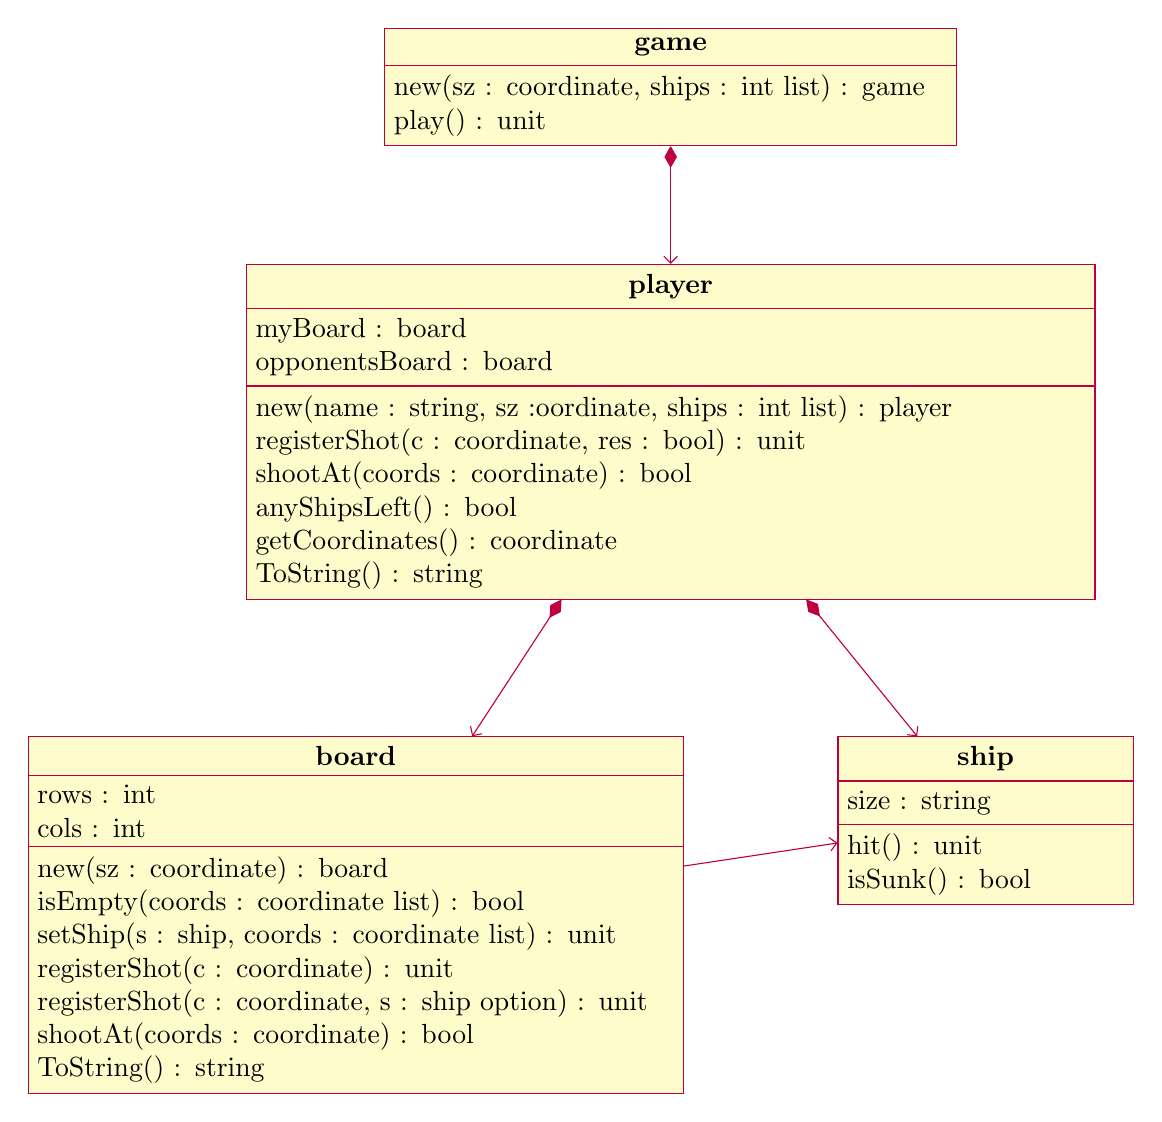
\begin{tikzpicture}
  \begin{class}[text width=20em]{game}{0,0}
    \operation{new(sz : coordinate, ships : int list) : game}
    \operation{play() : unit}
  \end{class}
  \begin{class}[text width=30em]{player}{0,-3}
    \attribute{myBoard : board}
    \attribute{opponentsBoard : board}
    \operation{new(name : string, sz :oordinate, ships : int list) : player}
    \operation{registerShot(c : coordinate, res : bool) : unit}
    \operation{shootAt(coords : coordinate) : bool}
    \operation{anyShipsLeft() : bool}
    \operation{getCoordinates() : coordinate}
    \operation{ToString() : string}
  \end{class}
  \begin{class}[text width=23em]{board}{-4,-9}
    \attribute{rows : int}
    \attribute{cols : int}
    \operation{new(sz : coordinate) : board}
    \operation{isEmpty(coords : coordinate list) : bool}
    \operation{setShip(s : ship, coords : coordinate list) : unit}
    \operation{registerShot(c : coordinate) : unit}
    \operation{registerShot(c : coordinate, s : ship option) : unit}
    \operation{shootAt(coords : coordinate) : bool}
   \operation{ToString() : string}
   \end{class}
   \begin{class}[text width=10em]{ship}{4,-9}
    \attribute{size : string}
    \operation{hit() : unit}
    \operation{isSunk() : bool}
   \end{class}
  \composition{game}{}{}{player}
  \composition{player}{}{}{board}
  \composition{player}{}{}{ship}
  \unidirectionalAssociation{board}{}{}{ship}
\end{tikzpicture}
\end{document}

